\section{System Block Diagram}

\tikzset{
    block/.style = {
        rectangle, 
        rounded corners, 
        minimum width=3cm, 
        minimum height=1cm, 
        align=center, 
        draw=black, 
        fill=white
    },
    subblock/.style = {
        rectangle, 
        minimum width=1.5cm, 
        minimum height=0.7cm, 
        align=center, 
        draw=black, 
        fill=white
    },
    arrow/.style = {
        thick, 
        -{Stealth[scale=1.2]}
    }
}

\begin{tikzpicture}[node distance=1.2cm]

% UAV System
\node[block, minimum width=7cm, minimum height=3cm] (uav) {UAV};
    \node[subblock] (pi) at ([xshift=0cm, yshift=0cm]uav.north west) {RPi};
    \node[subblock] (camera) at ([xshift=0cm, yshift=0cm]uav.south west) {Camera};
    \node[subblock] (receiver) at ([xshift=0cm, yshift=-1.5cm]uav.north east) {Receiver\\Control};

% Ground System (to the left/west of UAV)
\node[block, right=4cm of uav] (ground) {Ground\\Transmitter};

% Image Upscaling just below Camera
\node[block, below=2cm of uav] (upscale) {Image Upscaling\\(Deep Learning)};

% Land Use Classification below Image Upscaling
\node[block, below=of upscale] (classify) {Land Use\\Classification};
\node[block, below=of classify] (analysis) {Result\\Analysis};

% Data Flow
\begin{scope}[arrow]
    \draw (ground.west) -- (receiver.east); % straight line
    \draw (uav.south) -- node[right, xshift=0.2cm] {Raw\\Images} (upscale.north);
    \draw (upscale) -- (classify);
    \draw (classify) -- (analysis);
\end{scope}

% Legend

\node[align=center] at ($(analysis.south) + (0,-1)$) 
    {\footnotesize \textbf{Figure~\thefigure: System Block Diagram of UAV System}};

\end{tikzpicture}
 
\subsection{System Description}

The system consists of a fixed-wing UAV platform equipped with essential components for flight and data collection. The UAV includes:

\begin{itemize}
    \item \textbf{ESC (Electronic Speed Controller):} Regulates the speed of the motor driving the propeller.
    \item \textbf{Propeller:} Provides thrust for UAV flight.
    \item \textbf{4 Servos:} Control the movement of aerodynamic surfaces like ailerons, elevator, and rudder for flight maneuverability.
    \item \textbf{Battery:} Powers the entire onboard system.
    \item \textbf{UAV Receiver:} Receives control signals from the ground-based transmitter.
    \item \textbf{Raspberry Pi + Camera Module:} Captures aerial images during flight.
\end{itemize}

The ground transmitter sends flight control commands to the UAV receiver. The Raspberry Pi processes input from the onboard camera and stores captured images.

These images are then passed to the image upscaling module using deep learning methods, enhancing the resolution and clarity. The upscaled images are further processed through a classification model to identify land use categories.
Finally, the results from the classification are analyzed for insights, contributing to high-resolution land use mapping from UAV-acquired data.

\section{Flowchart}
\begin{center}
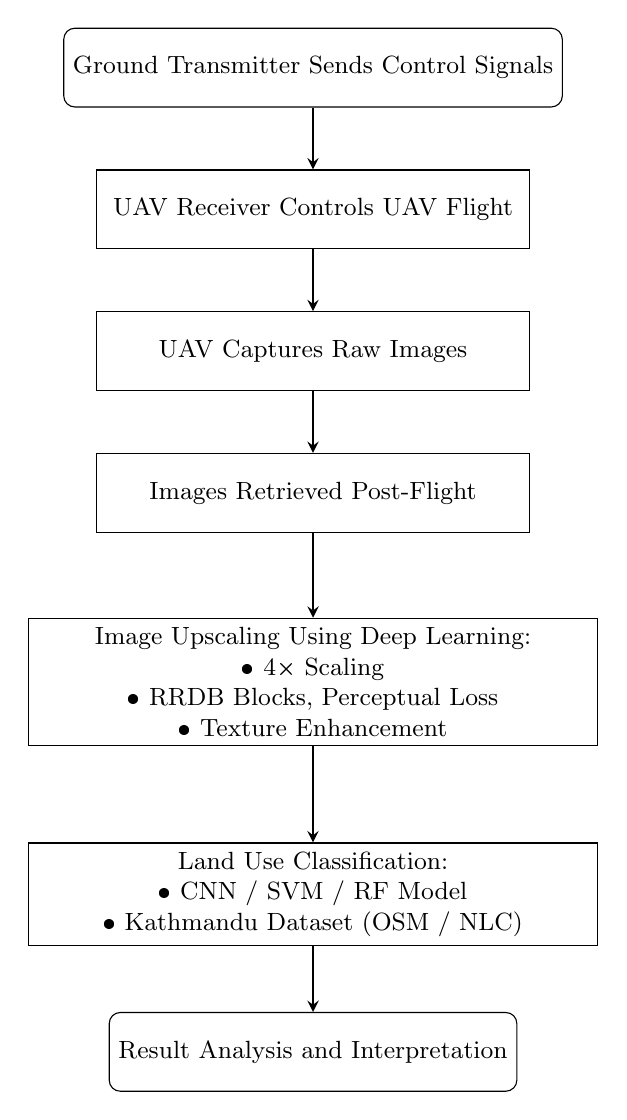
\begin{tikzpicture}[node distance=1.8cm, every node/.style={font=\small}] % increased node distance

\tikzstyle{startstop} = [rectangle, rounded corners, minimum width=3.5cm, minimum height=1cm, text centered, draw=black, fill=white]
\tikzstyle{process} = [rectangle, minimum width=5.5cm, minimum height=1cm, text centered, draw=black, fill=white]
\tikzstyle{arrow} = [thick,->,>=stealth]

\node (tx) [startstop] {Ground Transmitter Sends Control Signals};
\node (rx) [process, below of=tx] {UAV Receiver Controls UAV Flight};
\node (cam) [process, below of=rx] {UAV Captures Raw Images};
\node (ret) [process, below of=cam, yshift=-0cm] {Images Retrieved Post-Flight};
\node (upscale) [process, below of=ret, yshift=-0.6cm, text width=7cm] {
Image Upscaling Using Deep Learning:\\
• 4× Scaling\\
• RRDB Blocks, Perceptual Loss\\
• Texture Enhancement
};
\node (classify) [process, below of=upscale, yshift=-0.9cm, text width=7cm] {
Land Use Classification:\\
• CNN / SVM / RF Model\\
• Kathmandu Dataset (OSM / NLC)
};
\node (result) [startstop, below of=classify,yshift=-0.2cm] {Result Analysis and Interpretation};

% Arrows
\draw [arrow] (tx) -- (rx);
\draw [arrow] (rx) -- (cam);
\draw [arrow] (cam) -- (ret);
\draw [arrow] (ret) -- (upscale);
\draw [arrow] (upscale) -- (classify);
\draw [arrow] (classify) -- (result);

\end{tikzpicture}
\end{center}
